\documentclass[12pt]{article}
\newcommand{\bottomMargin}{2cm}

\newcommand{\header}{
	ДИЗАЙН И АНАЛИЗ НА АЛГОРИТМИ - \\ ПРАКТИКУМ\\
	\vspace{0.1cm}
        Летен семестър, 2025 г., контролно 1\\
	\vspace{0.1cm}
}
\newcommand{\tl}{$0,1$ сек.}
\newcommand{\ml}{$256$ MB}

%---DOCUMENT MARGINS---
\usepackage{geometry} % Required for adjusting page dimensions and margins
\geometry{
	paper=a4paper, % Paper size, change to letterpaper for US letter size
	top=4cm, % Top margin
	bottom=\bottomMargin, % Bottom margin
	left=2cm, % Left margin
	right=2cm, % Right margin
	headheight=3cm, % Header height
	%footskip=1.5cm, % Space from the bottom margin to the baseline of the footer
	headsep=0.5cm, % Space from the top margin to the baseline of the header
	%showframe, % Uncomment to show how the type block is set on the page
}
\usepackage{cmap}

\usepackage[T2A]{fontenc}
\usepackage[bulgarian]{babel}
\usepackage{fontspec}
\setmainfont{Times New Roman}
\setsansfont{Times New Roman}
\setmonofont{Courier New}
\usepackage[math-style=TeX]{unicode-math}
\setmathfont{Latin Modern Math}

\usepackage[nobottomtitles*]{titlesec}
\titleformat
{\section} % command
{\normalfont\fontsize{14}{14}\sffamily\bfseries} % format
{} % label
{0pt} % sep
{} % before-code
\titlespacing{\section}{0pt}{0em}{0em}
\usepackage[dvipsnames]{xcolor}
\titleformat
{\subsection} % command
{\fontsize{14}{14}\itshape} % format
{} % label
{0pt} % sep
{} % before-code
[\vspace{-1em}{\color{BrickRed}\rule{0.2\textwidth}{0.2em}}\vspace{-0.7em}] % after-code
\titlespacing{\subsection}{0pt}{0.5em}{0em}

\setlength{\parskip}{0.5em}
\setlength{\parindent}{24pt}
\sloppy

\usepackage{fancyhdr}
\pagestyle{fancy}
\usepackage{setspace}
\fancyhead[L]{
	\begin{minipage}{\textwidth}
		
\includegraphics[width=2.8cm]{/structure/logo.png}
	\end{minipage}
}
\fancyhead[C]{
	\begin{minipage}{\textwidth}
		\centering\large{\bf{\header}}
		\vspace{-0.35cm}
	\end{minipage}
}
\usepackage{emoji}
\usepackage{makecell}
\usepackage{tabularray}
\AtBeginEnvironment{table}{\vspace{-0.2cm}}
\AtEndEnvironment{table}{\vspace{-0.2cm}}
\usepackage{float}
\fancyhead[R]{
	\begin{tabular}{r@{\hspace{0.2cm}}l}
		\emoji{hourglass-not-done}: & \tl \\ 
		\emoji{floppy-disk}: & \ml \\ 
	\end{tabular}%
}
\renewcommand{\headrulewidth}{0cm}
\fancyheadoffset[L]{1cm}
\fancyheadoffset[R]{1cm}

\raggedbottom

\usepackage{amsmath}
\usepackage{stmaryrd}

\usepackage{graphicx}
\graphicspath{{./}}
\usepackage[export]{adjustbox}
\usepackage{wrapfig}
\makeatletter
\patchcmd\WF@putfigmaybe{\lower\intextsep}{}{}{\fail}
\AddToHook{env/wrapfigure/begin}{\setlength{\intextsep}{0pt}}
\makeatother
\usepackage[inkscapearea=page,inkscapepath=./svg-inkscape]{svg}
\svgpath{{./}}

\usepackage{placeins}
\usepackage{caption}
\captionsetup[table]{
	skip=0.25em,font=it,
	singlelinecheck=false,justification=justified,indention=-24pt,
	margin={24pt, 0pt}
}

\usepackage{enumitem}
\setlist{itemsep=-0.4em,leftmargin=\parindent,topsep=-\parskip}
\newcommand{\tabitem}{\indent~~\llap{\textbullet}~~}

\usepackage{hyperref}
\hypersetup{
	colorlinks=true,
	citecolor=blue,
	linkcolor=blue,
	urlcolor=cyan,
}


\begin{document}
\section{Задача К2. Ескейп}
\begin{wrapfigure}{r}{0.5\textwidth}
    \centering
    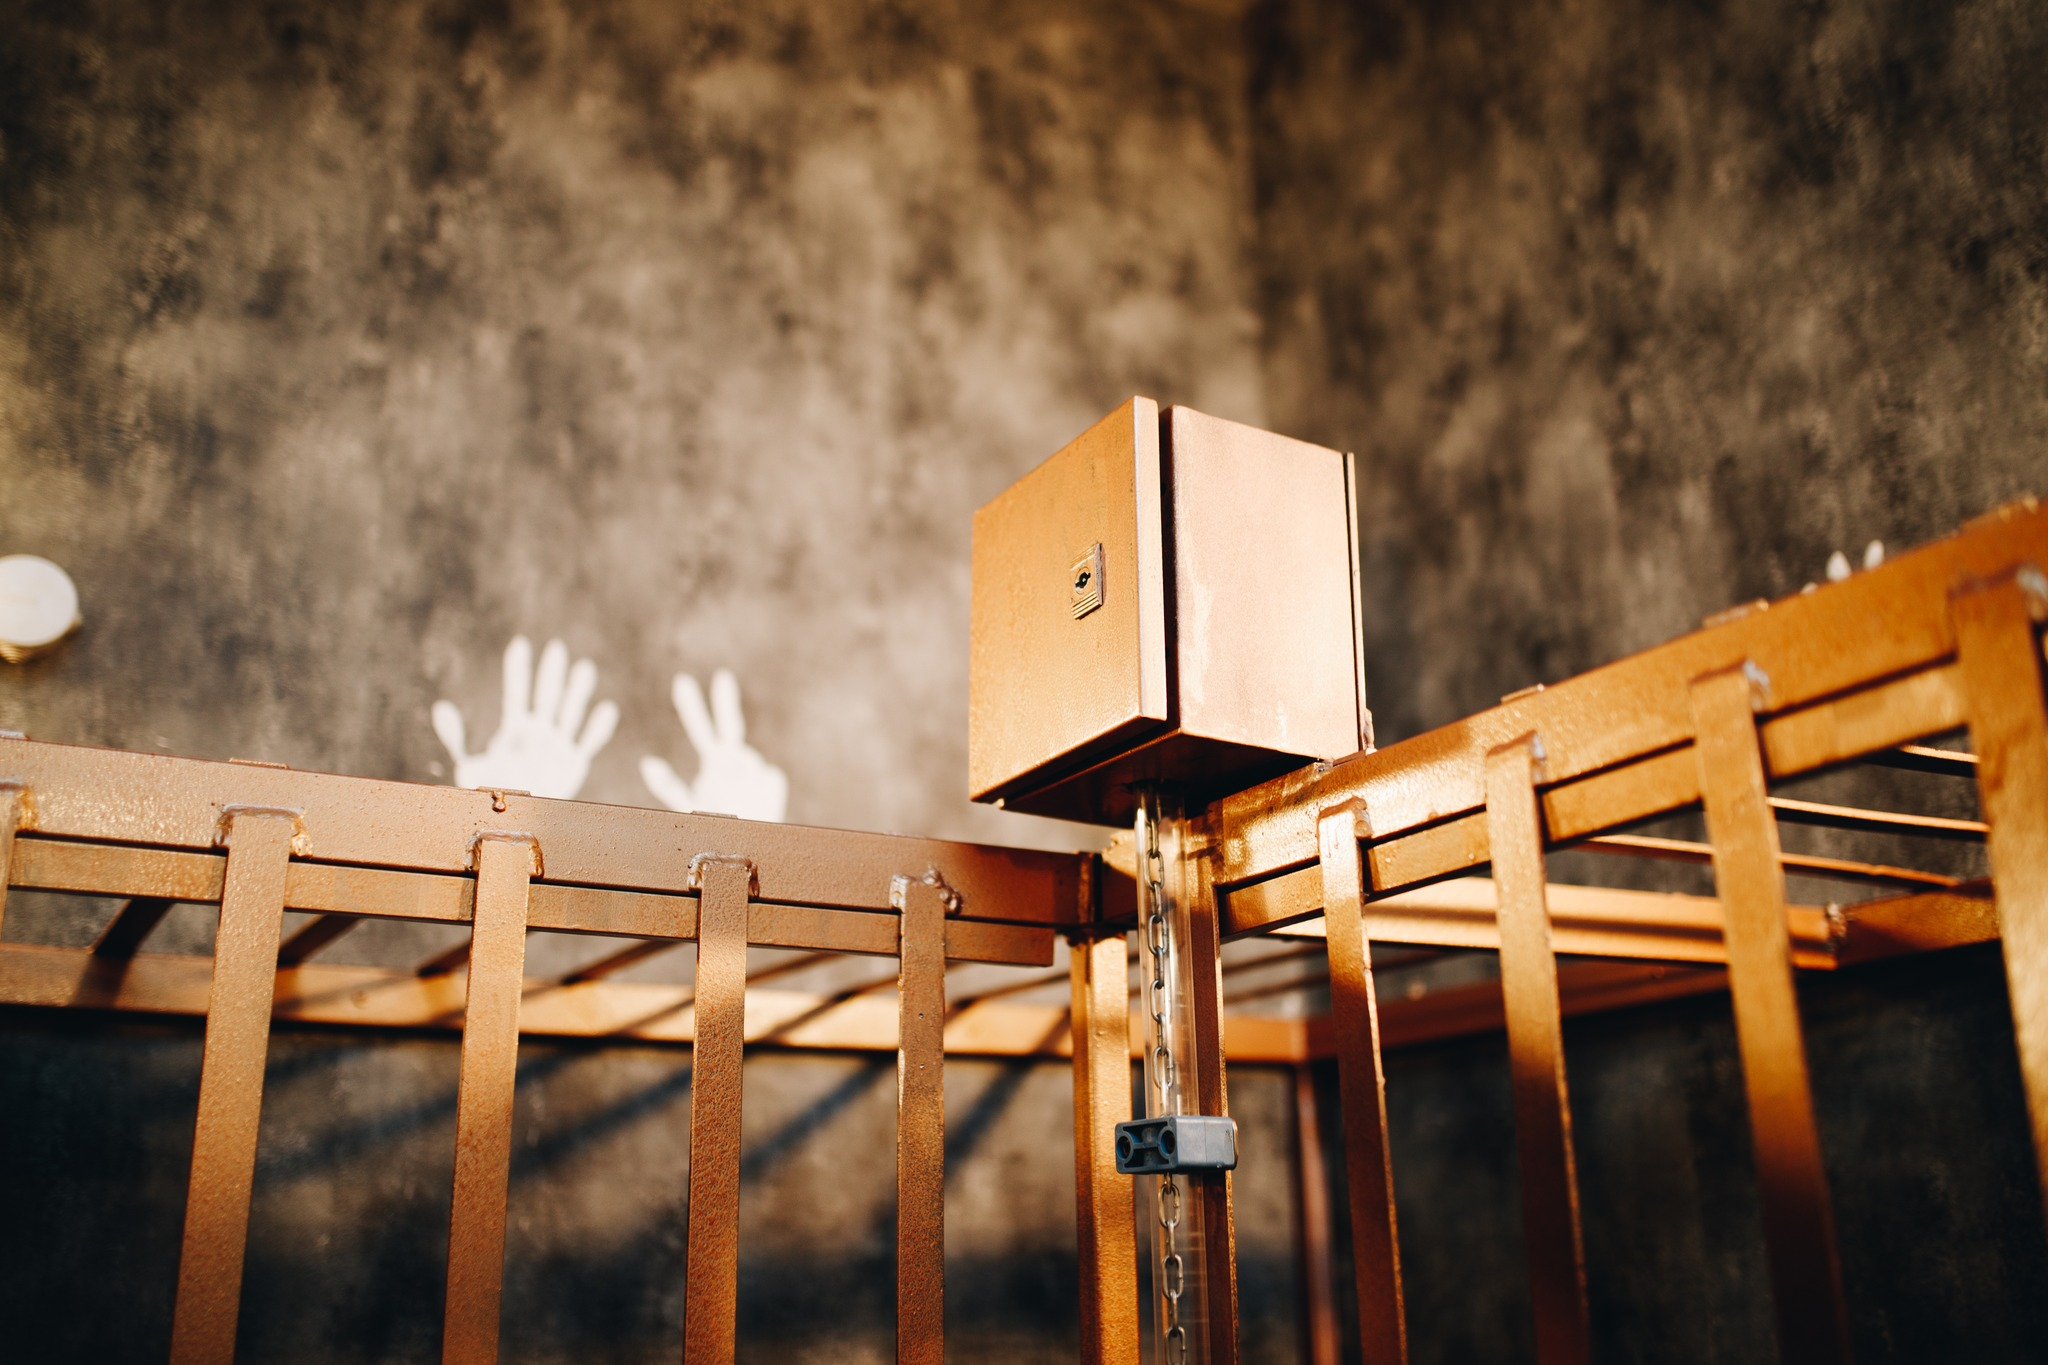
\includegraphics[width = 8.5cm]{structure/escape_image.png}
\end{wrapfigure}
Теодор е решил да пробва най-новата ескейп стая в града. В момента той се намира в помещение с N врати, всяка водеща към различна стая. Във всяка стая има по един контейнер с вода. По-точно, в стая $i$ има контейнер, съдържащ $l_i$ литра вода. До $i$-тия контейнер има туба, чийто обем е $t_i$ литра. Всяка туба е закачена с верига за стената, така че да не може бъде изнасяна от съответната стая. За какво се използва всичко това, така и не става ясно, но това не вълнува особено Теодор в момента. Той вече не мисли за това как да реши пъзела, а как да всее хаос. Неговият план е да покаже на създателите на ескейп стаята защо е лоша идея да слагат вода в нея.

Теодор разполага с $K$ мунити. За всяка минута той отива до някоя стая, в която пълни съответната туба с вода. Не е задължително тубата да бъде напълнена догоре, но е важно да има поне толкова литра останали в контейнера. След това той излива съдържанието й на пода. За да заблуждава гейм-мастърите, които гледат през камерите, Теодор всяка минута се връща до главното помещение.

Помогнете на Теодор като напишете програма \textbf{escape}, която намира колко най-много литра може да излее след $K$ минути.
\subsection{Вход}
От първия ред на стандартния вход се въвеждат две цели числа - съответно $N$ и $K$. От следващите $N$ реда се въвеждат по две цели числа $l_i$ и $t_i$ – съответно обема на контейнера и тубата в $i$-тата стая.

\subsection{Изход}
На първия ред на стандартния изход изведете едно цяло число – максималният брой литри, които Теодор може да излее.

\subsection{Ограничения}
\begin{itemize}
	\item $1\leq N \leq 100\ 000$
    \item $1\leq K \leq 10^{14}$
    \item $1\leq l_i, t_i \leq 10^9$
    %\item В ??? процента от тестовете $1\leq N, M \leq 10^3$
\end{itemize}

\subsection{Пример}
\begin{table}[H]
	\begin{tblr}{|X[12,l]|X[8,l]|X[80,j]|}
		\hline
		\textbf{Вход} & \textbf{Изход} & \textbf{Обяснение на примера} \\
		\hline
		\texttt{3 5 \\
10 4 \\
2 1 \\
13 5 \\
}
		& 
		\texttt{21}
		& 
		{Теодор може да разпредели времето си по следния начин: \\
        $2$ минути за стая $1$ \\
        $3$ минути за стая $3$ \\
        } \\
		\hline
        \texttt{6 21 \\
18 4 \\
30 7 \\
29 5 \\
13 4 \\
3 1 \\
9 3 \\
}
		& 
		\texttt{96}
		& 
		{Теодор може да разпредели времето си така: \\
        $4$ минути за стая $1$ \\
        $5$ минути за стая $2$ \\
        $6$ минути за стая $3$ \\
        $3$ минути за стая $4$ \\
        $3$ минути за стая $6$ \\
        } \\
		\hline
	\end{tblr} 
\end{table}
\FloatBarrier

\end{document}
